\documentclass{article}
\usepackage[utf8]{inputenc}
\usepackage{amsmath, listings, textcomp, xcolor, graphicx, verbatim, bm}
\usepackage[document]{ragged2e}
\usepackage{amssymb} %in order to get real-numbers, natural etc. 
\usepackage{tikz} %generated plots from csv. 
\usepackage{thmtools}
\usepackage{enumerate} %lists
\usepackage{pgfplots} 
\usepackage{color}   %May be necessary if you want to color links
\usetikzlibrary{datavisualization} %something for plotting
\usepackage{hyperref}
\hypersetup{
    colorlinks=true, %set true if you want colored links
    linktoc=all,     %set to all if you want both sections and subsections linked
    linkcolor=blue,  %choose some color if you want links to stand out
}
%Referencing
\usepackage[utf8]{inputenc}
\usepackage[english]{babel}

\usepackage{biblatex}
\addbibresource{references.bib}



\lstset{
	backgroundcolor=\color[rgb]{0.95,0.95,0.95},
	tabsize=4,
	rulecolor=,
	language=python,
      basicstyle=\scriptsize,
      upquote=true,
      aboveskip={1.5\baselineskip},
      columns=fixed,
      showstringspaces=false,
      extendedchars=true,
      breaklines=true,
      prebreak = \raisebox{0ex}[0ex][0ex]{\ensuremath{\hookleftarrow}},
      frame=single,
      showtabs=false,
      numbers=left,
      showspaces=false,
      showstringspaces=false,
      identifierstyle=\ttfamily,
      keywordstyle=\color{blue},
      commentstyle=\color{green},
      stringstyle=\color{black}
}
\newcommand{\R}{\mathbb{R}}
\newcommand{\N}{\mathbb{N}}
\newcommand{\A}{\mathcal{A}}
\newcommand{\G}{\mathcal{G}}
\newcommand{\F}{\mathcal{F}}
\newcommand{\Abar}{\overline{\mathcal{A}}}
\newcommand{\Rbar}{\overline{\mathbb{R}}}%the extended real numbers.
\newcommand{\mubar}{\overline{\mu}}
\newcommand{\Null}{\mathcal{N}}
\newcommand{\B}{\mathcal{B}}
\newcommand{\I}{\mathcal{I}}
\newcommand{\Q}{\mathbb{Q}}
%\newcommand{\P}{\mathcal{P}}



\newtheorem{definition}{Definition}
\newtheorem{prop}{Proposition}
\newtheorem{ex}{Example}
\newtheorem{lemma}{Lemma}
\newtheorem{proof}{Proof}
\newtheorem{theorem}{Theorem}
\newtheorem{result}{Result}
\newtheorem{cor}{Corollary}

\title{Measure theory}
\author{Andreas Slaattelid}
\date{} 



\begin{document}
\maketitle  
\tableofcontents
These are lecture notes based on MAT4400 – Linear Analysis with Applications, they are mainly based on \cite{LindstrømSpaces}, as well as Tom Lindstrøm's excellent notes himself from classes. 

\newpage
\section{An introduction to measure theory}

\subsection{Sigma-algebras and measures}

\begin{definition}[sigma-algebra]
Assume that $X$ is a non-empty set, a family $\A$ of subsets of $X$ is called a sigma-algebra if the following holds: 
\begin{enumerate}[i)]
  \item $\emptyset \in \A$
  \item If $A\in \A$, then $A^{C}\in \A$ 
  \item If $A_{n} \in \A$ for all $n\in \N$, then $\bigcup_{n\in \N}A_{n}\in \A$
\end{enumerate}
\end{definition}

\begin{prop}
Assume that $\A$ is a sigma-algebra on $X$, then the following holds: 
\begin{enumerate}[i)]
    \item $X\in \A$
    \item if $\{A_{n}\}_{n\in \N} \in \A$, then $\bigcap_{n\in \N}A_{n} \in \A$
    \item if $A_{1}, \dots A_{n} \in \A$, then $\bigcup_{k=1}^{n}A_{k} \in \A$ and $\bigcap_{k=1}^{n}A_{k} \in \A$
    \item if $A,B \in \A$, then $A\setminus B \in \A$
\end{enumerate}
\end{prop}

This is a useful proposition, and are not included in the definition since it actually follows from the definition. 

\begin{definition}[measure]
Assume that $X$ is a non-empty set, and that $\A$ is a $\sigma$-algebra on $X$. \\ 
A measure $\mu$ on $(X,\A)$ is a function $\mu:\A\to \overline{\R}_{+} =[0,\infty)\cup \{\infty\}$ such that: 
\begin{enumerate}[i)]
    \item $\mu(\emptyset) = 0$ 
    \item if $\{A_{n}\}_{n\in \N}$ is a pairwise disjoint sequence, then: 
    $\mu\left(\bigcup_{n\in \N}A_{n}\right) = \sum_{n\in \N}\mu(A_{n})$ 
\end{enumerate}
We call the triplet $(X,\A,\mu)$ a measure space.
\end{definition}

When we know what a measure and a sigma-algebra is, then we are ready for examples of measures, and see why in fact we can call them measures:  

\begin{ex}[Counting measure]
This is the counting measure, also known as the cardinality of a set: let $X = \{x_{1}, \dots, x_{n}\}$ be a finite set, and let $\A = \mathcal{P}(X)$, then: $\mu(A) = |A|$ is a measure on $X$. \\ 
Why is this a measure? First of all we have that the set $X$ is finite, so for all sets $A\in \mathcal{P}(X)$ we will have $|A| < \infty$, as well as $|A| \geq 0$. this means that $\mu$ takes values in $[0, \infty)$ which is a requirement for a measure. And by definition we also have that $\mu(\emptyset) = |\emptyset| = 0$ (the empty set has zero elements).\\ 
We also have that for the disjoint sequence $\{A_{n}\}_{n\in \N}$: $\mu\left(\bigcup_{n\in \N}\right) = \left|\bigcup_{n\in \N}A_{n} \right|
= \sum_{n\in \N}|A_{n}| = \sum_{n\in \N}\mu(A_{n})$. 
Hence the counting measure is indeed a measure.
\end{ex}  

\begin{ex}[Dirac measure]
We here have one rather simple measure, but actually one of the most important ones, and it looks like this: 
\[ \mu(A) = \delta_{x}(A) =  \begin{cases}
      1 & x \in A\\
      0 & x \not\in A
    \end{cases} 
\] 
We have that the measure takes only 1 or 0 as values,\\
so we have that $\mu(A) \geq 0, \forall A\in \A$, we also have that $\mu(\emptyset) = 0$, this is because by definition $x\not\in \emptyset$. \\
Before we generalize, lets assume the following: 
\begin{align*}
X = \{a_{1},a_{2}\}\;\; \mathcal{P}(X) = \{\emptyset, \{a_{1}\}, \{a_{2}\}, \{a_{1}, a_{2}\}\} = \{A_{1}, A_{2}, A_{3}, A_{4}\} \\ 
\text{our disjoint sets here are:}\;\; A_{1}, A_{2}, A_{3}\;\; \text{so this means that:}\\ 
x \in \bigcup_{k=1}^{3}A_{k} = \{x\in A_{1} \;or\; x\in A_{2} \;or\; x\in A_{3}\} \\ 
x \in \bigcup_{k=1}^{3}A_{k} \implies \mu\left(\bigcup_{k=1}^{3} A_{k}\right) = 1 = \sum_{k=1}^{3}\mu(A_{k}) = 0 + 1 + 0 \;\;(x\in A_{2})
\end{align*}
And with the above intuition we can generalize: let $\{A_{n}\}_{n\in \N}$ be a pairwise disjoint sequence, for some $m\in \N$, we will have $x\in A_{m}$ and for $n\neq m$, we will have $x\not\in A_{n}$, which means that: 
\[\mu\left(\bigcup_{n\in \N}A_{n}\right) = 1 = \sum_{n\in \N}\mu(A_{n}) = 0 + 0+\dots + \mu(A_{m}) + 0 + \dots = 1
\] 
In the other case, i.e where $x \not\in A_{n} \; \forall n\in \N$ we have: 
\[\mu\left(\bigcup_{n\in \N}A_{n}\right) = 0 = \sum_{n\in \N}\mu(A_{n})
\] 
Hence the Dirac measure is a measure 
\end{ex} 

\newpage
\begin{ex}[sigma-algebra of countable sets and measure]
Let $X$ be an uncountable set, and define the sigma-algebra\\ 
$\A = \{A \in \mathcal{P}(X): A\; is\; countable\; or\; A^{C}\; is\;countable\}$ as well as the measure: 
\[ \mu(A) = \begin{cases}
      0 & \text{if  $A$ is countable}\\
      1 & \text{if  $A^{C}$ is countable}
    \end{cases}    
\]
We can start by verifying that $\A$ is a $\sigma$-algebra: We have that $\emptyset \in \mathcal{P}(X)$, and by definition we have that the $\emptyset$ is countable, hence $\emptyset \in \A$.\\ 
We also want to have that $A\in \A \implies A^{C}\in \A$: so assume that $A$ is countable, i.e an element of $\A$ and let $B=A^{C}$, we will then have that\\ $B^{C} = (A^{C})^{C} = A$, hence we must have that $A^{C}$ is an element of $\A$, since it's complement is countable.\\ 
We must also show that: $A_{1}, \dots A_{n} \in \A \implies \bigcup_{k=1}^{n}A_{k} \in \A$. let's start with the simplest case where all $A_{k}$ is countable, then we have by definition that $\bigcup_{k=1}^{n}A_{k}$ is countable, hence also in $\A$. \\ 
In our second case it could be that they are not countable, i.e maybe all or some of them, but assume that there exist $i\in \N$ s.t $A_{i}^{C}$ is countable. Then we will have: $(\bigcup A_{n})^{C} = \bigcap A_{n}^{C} \subseteq A_{i}^{C}$. This is easiest understood by venn diagrams: 
\\
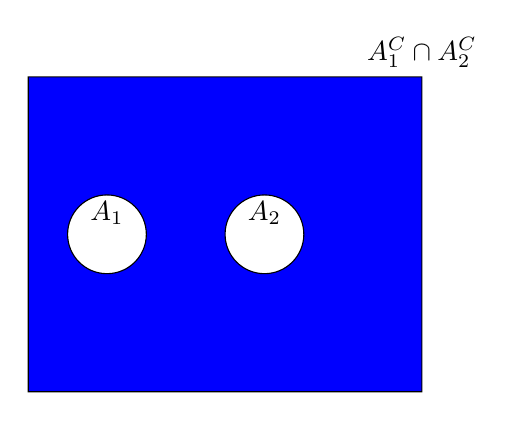
\begin{tikzpicture}

\def\bigrectangle{(-2,-2) rectangle (3,2)}
\def\firstcircle{(-1,0) circle (0.5)}
\def\secondcircle{(1,0) circle (0.5)}

% fill rectangle and conjunction
\scope
    \clip \firstcircle \secondcircle \bigrectangle;
    \fill[blue] \bigrectangle;
\endscope

% fill conjunction white
\scope
    \clip \secondcircle;
    \fill[white] \firstcircle;
\endscope

% outline
\draw \firstcircle (-1,0) node [text=black,above] {$A_{1}$}
      \secondcircle (1,0) node [text=black,above] {$A_{2}$}
      \bigrectangle node [text=black,above] {$A_{1}^{C}\cap A_{2}^{C}$};

\end{tikzpicture}


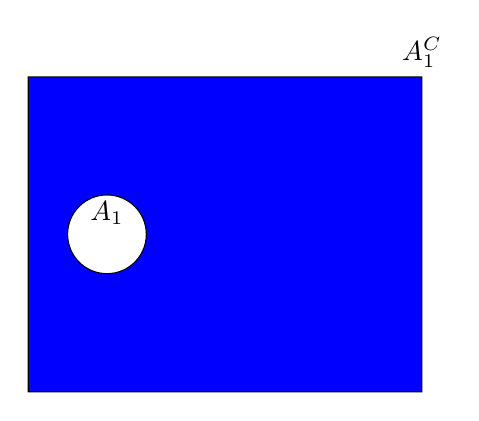
\begin{tikzpicture}

\def\bigrectangle{(-2,-2) rectangle (3,2)}
\def\firstcircle{(-1,0) circle (0.5)}
%\def\secondcircle{(1,0) circle (0.5)}

% fill rectangle and conjunction
\scope
    \clip \firstcircle  \bigrectangle;
    \fill[blue] \bigrectangle;
\endscope

% fill conjunction white
\scope
    %\clip \secondcircle;
    \fill[white] \firstcircle;
\endscope

% outline
\draw \firstcircle (-1,0) node [text=black,above] {$A_{1}$}
      %\secondcircle (1,0) node [text=black,above] {$A_{2}$}
      \bigrectangle node [text=black,above] {$A_{1}^{C}$};

\end{tikzpicture}

The idea here is that the blue area in the last figure is larger than the blue area in the first figure, hence $A_{1}^{C}\cap A_{2}^{C} \subseteq A_{1}^{C}$
Now we have finally shown that $\A$ is a sigma-algebra, we now only have to show that $\mu$ is indeed a measure.
\newpage 
$\mu(\emptyset) = 0$, since $\emptyset$ is countable. \\ 
Now again let all sets $A_{1},\dots, A_{n}$ be countable pairwise disjoint. hence:\\ 
$\mu\left(\bigcup_{k=1}^{n}A_{k}\right) = 0 = \sum_{k=1}^{n}\mu(A_{k})$, again this holds since the union is countable.\\ 
Now we look at a less ideal situation, namely maybe not all sets are countable. Let $A = \bigcup_{n\in \N}A_{n}$, and assume that there exist atleast one $m\in \N$, such that $A_{m}^{C}$ is countable. So we have then that $A^{C}\subseteq A_{m}^{C}$, this is easiest understood by drawings, but as $A_{m}^{C}$ is just one countable set, we will have that the union $A^{C} = (\bigcup_{n\in \N}A_{n})^{C}$ is a smaller set than $A_{m}^{C}$. But this means that $A^{C}$ is a countable set, as it is a subset of a countable set, hence $A\in \A$ (since $A^{C}\in \A)$.\\ 
We still assume that $\{A_{n}\}_{n\in \N}$ is a disjoint sequence, this means that:\\
$A_{n}\subseteq A_{m}^{C}, \; n\neq m$. So for $n\neq m$ we have that $A_{n}$ is countable. 
\begin{align*}
\sum_{n\in \N}\mu(A_{n}) &= \sum_{n\neq m}\mu(A_{n}) + \mu(A_{m})\\ 
                         &= 0 + 1 = 1 \;\;(A_{m}^{C} \; is \; countable)  \\ 
\mu\left(\bigcup_{n\in \N}A_{n}\right) &= 1 \\ 
\mu\left(\bigcup_{n\in \N}A_{n}\right) &= 1 = \sum_{n\in \N}\mu(A_{n})
\end{align*}
\end{ex}

\begin{prop}
Let $(X,\A, \mu)$ be a measure space, then we have: 
\begin{enumerate}[i)]
    \item (Finite addativity) if $A_{1}, \dots, A_{m}$ are disjoint sets in $\A$, then: $$\mu\left(\bigcup_{n=1}^{m}A_{n}\right) = \sum_{n=1}^{m}\mu(A_{n})$$
    \item (Monotinicity) if $A,B \in \A$, and $A\subseteq B$, with $\mu(B) < \infty$, then:\\ $\mu(A)\leq \mu(B)$ 
    \item if $A,B\in \A$, with $A\subseteq B$ and $\mu(B) < \infty$, then: \\
    $\mu\left(A\setminus B\right) = \mu(B) -\mu(A)$ 
    \item (Subaddativity) let $\{A_{n}\}_{n\in \N}$ be a sequence in $\A$, not necessarily disjoint, then: 
    \[\mu\left(\bigcup_{n\in \N}A_{n}\right) \leq \sum_{n\in \N}\mu(A_{n})
    \]
\end{enumerate}
\end{prop}

The idea again, is to use the definition of the measure to verify these, so for $i)$ we just supply the sequence with empty-sets. $iii)$ is a consequence of $ii)$ and $iv)$ is a consequence of defintion again: 

\begin{proof}
We start with ii): 
\begin{align*}
B &= A\cup(B\setminus A)\; (disjoint) \\
\mu(B) &= \mu(A) + \mu(B\setminus A)\\ 
 &\geq \mu(A)
\end{align*} 
iii) follows directly from above, just reorder the equation. \\ 
iv): Let $\{A_{n}\}$ be the sequence in $\A$ not necessarily disjoint. We want to create a disjoint set of these sets namely $\{B_{n}\}$
\begin{align*}
B_{1} = A_{1}, \;\;B_{2}=A_{2}\setminus B_{1},\;\; B_{3} = A_{3}\setminus(B_{1}\cup B_{2}),\dots, B_{n}= A_{n}\setminus(\bigcup_{k=1}^{n-1}B_{k})\\ 
\mu(\bigcup_{n\in \N}A_{n}) = \mu(\bigcup_{n\in \N}B_{n}) = \sum_{n\in \N}\mu(B_{n}) \leq \sum_{n\in \N}\mu(A_{n})\; (\text{by monotinicity: $B_{n}\subseteq A_{n}$})
\end{align*}
\end{proof}

\begin{prop}[Continuity of measure]
Let $\{A_{n}\}_{n\in \N}$ be a sequence of measurable sets in $(X, \A, \mu)$, then we have: 
\begin{enumerate}[i)]
    \item Assume that $\{A_{n}\}_{n\in \N}$ is an increasing sequence, i.e that $A_{n} \subseteq A_{n+1}$ for all $n\in \N$, then: 
    \[\mu\left(\bigcup_{n\in \N}A_{n}\right) = \lim_{n\to \infty}\mu(A_{n})
    \]
    \item Assume that $\{A_{n}\}_{n\in \N}$ is a decreasing sequence, i.e that $A_{n+1} \subseteq A_{n}$ for all $n\in \N$, and that $\mu(A_{1}) < \infty$ then: 
    \[\mu\left(\bigcap_{n\in \N}A_{n}\right) = \lim_{n\to \infty}\mu(A_{n})
    \]
\end{enumerate}
\end{prop}

\begin{proof}
We start by proving $i)$: let $A = \bigcup_{n\in \N}A_{n}$ and lets define a new disjoint sequence $\{B_{n}\}_{n\in \N}$ by: $B_{1} = A_{1}$, $B_{2} = A_{2}\setminus A_{1}, \dots B_{n} = A_{n}\setminus A_{n-1}$. This means that: 
\begin{align*}
\mu(A) = \mu(\bigcup_{n\in \N}B_{n}) = \sum_{n\in \N}\mu(B_{n}) = \lim_{m\to \infty}\sum_{n=1}^{m}\mu(B_{n}) = \lim_{m\to \infty}\mu\left(\bigcup_{n=1}^{m}B_{n}\right) = \lim_{m\to \infty}\mu(A_{m})    
\end{align*} 
For part two, we again want to define a disjoint sequence: let $B_{n} = A_{1}\setminus A_{n}$ so $\{B_{n}\}_{n\in \N}$ is an increasing sequence. And let $A = \bigcap_{n\in N}A_{n}$. We will then have that $\bigcup_{n\in \N}B_{n} = A_{1}\setminus \bigcap_{n\in \N}A_{n} = A_{1}\setminus A$
\end{proof}

\begin{ex}[Cont of measure]
Let $\mu$ be a measure on $\R$ such that\\
$\mu([-1/n,1/n]) = 1 + 2/n, n\in \N$, then we have $\mu(\{0\}) = 1$.\\ 
Define $A_{n} = [-1/n, 1/n]$ then we have that the sequence $\{A_{n}\}_{n\in \N}$ is decreasing ($A_{n+1}\subseteq A_{n}$. $\mu(A_{1}) = 1 + 2/1 = 3 < \infty$. As well as $\{0\} = \bigcap_{n\in \N}A_{n}$. Now since all the requirements for continuity of measure is fulfilled, we thus have: 
\[\mu(\{0\}) = \mu(\bigcap_{n\in \N}A_{n}) = \lim_{n\to \infty}\mu(A_{n}) 
= \lim_{n\to \infty} 1 + 2/n = 1
\]
\end{ex} 

\begin{ex}[When requirements does not hold]
Let $\mu$ be the Lesbegue measure on $\R$, i.e: $\mu([a,b]) = b-a$. Let's put $A_{n} = [n,\infty)$ so this means that $\mu(A_{n}) = \infty, \; \forall n\in \N$, thus $\lim_{n\to \infty}\mu(A_{n}) = \infty$. We have that $\{A_{n}\}$ is a decreasing sequence, with $\mu(A_{1}) = \infty$. We can also look at the intersection: $\bigcap_{n\in \N}A_{n} = \bigcap_{n\in \N}[n, \infty) = \emptyset$. Which again yields:\\ 
$\mu(\bigcap_{n\in \N}A_{n}) = \mu(\emptyset) = 0 \neq \lim_{n\to \infty}\mu(A_{n})$
\end{ex} 

\subsection{Complete measures}
We have until now defined what a sigma-algebra and a measure is, but the definition does not capture everything. Assume that $(X,\A,\mu)$ is a measurespace and let $B\in \A$ be such that $\mu(B)=0$, further assume that $N\subseteq B$, a question that arises is then: will $\mu(N) = 0$? If $N\in \A$, then we will have: $\mu(N) = 0$. This follows from the monotonicity property of the measure. The problem is when $N\not\in \A$, our defintion of the measure does not say anything about this. So in general we will have that $N$ does not need to be in $\A$. 

\begin{definition}[Null set]
A set $N\subseteq X$ is called a null set, if there is a set $B\in \A$ such that $N\subseteq B$ and $\mu(B) = 0$. 
\end{definition}

\begin{definition}[Complete measure space]
A measure space $(X,\A, \mu)$ is called complete if all null sets belongs to $\A$.
\end{definition}

The goal of this section is to turn an arbitrary measure space into a complete measure space. Before we continue, we denote $\mathcal{N}$ the collection of all null sets.

\begin{lemma}
If $N_{n}\in \mathcal{N}$, then: $\bigcup_{n\in \N}N_{n} \in \mathcal{N}$
\end{lemma}

\begin{proof}
Since $N_{n}$ is a null set, we have that there is a $B_{n}\in \A$ s.t\\ $N_{n}\subseteq B_{n}, \; \forall n\in \N$, with $\mu(B_{n}) = 0$. We will therefore have: $\bigcup_{n\in \N}N_{n} \subseteq \bigcup_{n\in \N}B_{n}$, and by subadditivity of measure: 
\[\mu\left(\bigcup_{n\in \N}B_{n}\right) \leq \sum_{n\in \N}\mu(B_{n}) = 0
\]
Hence $\bigcup_{n\in \N}N_{n} \in \mathcal{N}$
\end{proof}

\begin{prop}[Smallest sigma-algebra containg $\A$ and $\mathcal{N}$]
Let \\
$\overline{\A} = \{A\cup N: A\in \A\; and\; N\in \mathcal{N}\}$, then $\overline{\A}$ is the smallest $\sigma$-algebra containg $\A$ and $\mathcal{N}$. 
\end{prop}

\begin{proof}
We start by showing that $\overline{\A}$ contains $\A$ and $\mathcal{N}$: \\
$\A \subseteq \overline{\A}$:
\begin{align*}
A\in \A: A &= A\cup \emptyset \in \overline{\A}\; (A\in \A, \; \emptyset \in \mathcal{N})\\ 
N\in \mathcal{N}: N &= \emptyset \cup N \in \overline{\A}\; (\emptyset \in \A, \; N \in \mathcal{N})
\end{align*}
If we assume that $\overline{\A}$ is a $\sigma$-algebra, then it must be the smallest one containg $\A$ and $\mathcal{N}$ because any other $\sigma$-algebra $\G$ must have $A\cup N$ as an element, hence $\overline{\A}\subseteq \G$.
Now the last thing we need to show is that $\overline{\A}$ actually is a $\sigma$-algebra. 
\begin{align*}
\emptyset \in \overline{\A}: \emptyset = \emptyset\cup \emptyset \in \overline{\A} \\ 
A\cup N \in \overline{\A} \implies (A\cup N)^{C} \in \overline{\A}:\\ 
(A\cup N)^{C} = (A\cup B)^{C}\cup (B\setminus N) \in \overline{\A}\\ 
(A_{n}\cup N_{n}) \in \overline{\A}\; \forall n\in \N \implies \bigcup_{n\in \N}\left(A_{n}\cup N_{n}\right) \in \overline{\A}: \\ 
\bigcup_{n\in \N}\left(A_{n}\cup N_{n}\right) = \left(\bigcup_{n\in \N}A_{n}\right)\cup \left(\bigcup_{n\in \N}N_{n}  \right) \in \overline{\A}
\end{align*}
Thus $\overline{\A}$ is the smallest $\sigma$-algebra containg $\A$ and $\mathcal{N}$. 
\end{proof}  

\begin{lemma}
Assume that $A_{1}, A_{2} \in \A$ and $N_{1}, N_{2} \in \mathcal{N}$ and that: 
$A_{1}\cup N_{1} = A_{2}\cup N_{2}$, then: $\mu(A_{1}) = \mu(A_{2})$
\end{lemma}

\begin{proof}
Since $N_{2}$ is a null set, we have that $B_{2}\in \A$ with $N_{2}\subseteq B_{2}$ and $\mu(B_{2}) = 0$. But then: 
\begin{align*}
A_{1} &\subseteq A_{1}\cup N_{1} = A_{2}\cup N_{2} \subseteq A_{2}\cup B_{2}\\ 
\mu(A_{1}) &\leq \mu(A_{2}\cup B_{2}) \leq \mu(A_{2}) + \mu(B_{2}) = \mu(A_{2})\\ 
A_{2} &\subseteq A_{2}\cup N_{2} = A_{1}\cup N_{1} \subseteq A_{1}\cup B_{1}\\ 
\mu(A_{2}) &\leq \mu(A_{1}\cup B_{1}) \leq \mu(A_{1}) + \mu(B_{1}) = \mu(A_{1})
\end{align*}
Hence $\mu(A_{1}) = \mu(A_{2})$. 
\end{proof}

It may seem strange why we included this lemma, but the idea is that we want to define a measure $\overline{\mu}:\overline{\A}\to \overline{R}_{+}$ such that: $\overline{\mu}(A\cup N) = \mu(A)$, so if we have two equal unions: $A_{1}\cup N_{1} = A_{2}\cup N_{2}$, then: $\overline{\mu}(A_{1}\cup N_{1}) = \overline{\mu}(A_{2}\cup N_{2}) = \mu(A_{1}) = \mu(A_{2})$ this lemma ensures us that if we have two equal unions, then they have the same measure. 

\begin{theorem}[Complete measure space with complete measure]
Assume that $(X, \A, \mu)$ is a measure space, and let: $\Abar = \{A\cup N: A\in \A\; and\; N\in \Null \}$, define $\overline{\mu}:\Abar \to \Rbar_{+}$ by: 
\[\overline{\mu}(A\cup N) = \mu(A), \;\; \forall A\in \A
\]
Then $(X,\Abar, \overline{\mu})$ is a complete measure space extending $(X,\A,\mu)$. 
\end{theorem}

\begin{proof}
We first want to check that $\mubar$ is a measure
\begin{align*}
\mubar(\emptyset) &= 0: \\ 
\mubar(\emptyset) &= \mubar(\emptyset \cup \emptyset) = \mu(\emptyset) = 0
\end{align*}
Now let $\{C_{n}\}_{n\in \N}$ be a disjoint sequence in $(X, \Abar, \mubar)$, with $C_{n} = A_{n}\cup N_{n}$ we must show that : $\mubar(\bigcup_{n\in \N}C_{n}) = \sum_{n\in \N}\mubar(C_{n})$. First we notice that since the $C_{n}$'s are disjoint we must have that the $A_{n}$'s are disjoint. 
\begin{align*}
\sum_{n\in \N}\mubar(C_{n}) = \sum_{n\in \N}\mubar(A_{n}\cup N_{n}) 
= \sum_{n\in \N}\mu(A_{n}) = \mu\left(\bigcup_{n\in \N}A_{n}\right)
= \mubar\left(\bigcup_{n\in \N}(A_{n}\cup N_{n}) \right) 
= \mubar \left(\bigcup_{n\in \N} C_{n}\right)
\end{align*}

We therefore have that $\mubar$ is a measure. But why is this new measure space $(X, \Abar, \mubar)$ complete? There could be that we have some new null sets in $\Abar$, so we must therefore show that it is actually a complete measuresapce, i.e all null sets belongs to $\Abar$. \\ 
To prove that this new measure space is complete, we must show that if $M$ is a $\mubar$ null set, then $M\in \Abar$, which yields $\mubar(M) = 0$.  \\ 
$M$ a $\mubar$ null set: let $C\in \Abar$ such that $M\subseteq C$ with $\mubar(C) = 0$. Since $C \in \Abar$ we have that $C$ is on the form: $C = A\cup N$, with $N\in \Null$. But since $N\in \Null$, we know that there is a $B\in \A$ such that $N\subseteq B$ with $\mu(B) = 0$. This gives us: 
\begin{align*}
M \subseteq C = A\cup N \subseteq A \cup B\\ 
A\cup B \in \A \implies \mubar(A\cup B) = \mu(A\cup B), \;(\text{by definition})\\ 
0 = \mubar(C) \leq \mubar(A\cup B) = \mu(A\cup B) \leq \mu(A) + \mu(B) = 0\\ 
\mu(A) = 0: \mubar(C) = \mubar(A\cup N) = \mu(A) \implies \mubar(C) = \mu(A) = 0
\end{align*}
This means that $M \in \Null \subseteq \Abar$, hence the new measure $\mubar$ encaptures all null sets. 
\end{proof}

The main takeaway from this theorem is that we now have a way of turning arbitrary measure spaces $(X, \A, \mu)$ into complete measure spaces $(X, \Abar, \mubar)$. 

\begin{ex}[Measure space that is not complete]
Let $X = \{0,1,2\}$ and $\A = \{\emptyset, \{0,1\}, \{2\}, X\}$. We have the measure: $\mu: \A \to \Rbar_{+}$ defined by: $\mu(\emptyset) = \mu(\{0,1\}) = 0, \mu(\{2\}) = \mu(X) = 1$. We start by showing that $\A$ is a sigma-algebra: 
\begin{align*}
\emptyset &\in \A: \text{holds by defintion}\\ 
A &\in \A \implies A^{C} \in \A:\\ 
A_{1} &= \emptyset \implies A_{1}^{C} = X \in \A\\ 
A_{2} &= \{0,1\} \implies A_{2}^{C} = \{2\} \in \A \\ 
A_{3} &= \{2\} \implies A_{3}^{C} = \{0,1\} \in \A\\ 
\{A_{n}\}_{n\in \N} &\in \A \implies \bigcup_{n\in \N}A_{n} \in \A: \\ 
\bigcup_{n=1}^{4} A_{n} &= X \in \A
\end{align*} 
Thus $\A$ is a sigma-algebra. We also get that $\mu$ is a measure. But why is then the measure space $(X,\A, \mu)$ not complete? Notice that $\mu(\{0,1\}) = 0$ so if we call $B = \{0,1\}$ we have $\mu(B) = 0$, but here $N_{1} = \{0\}\in \Null$ and $N_{2} = \{1\} \in \Null$ and $N_{1}, N_{2} \not\in \A$, thus $(X,\A, \mu)$ is not complete. So how can we transform this into a complete measure space? By definition $\Abar = \{A\cup N: A\in \A \;and\; N\in \Null\}$, here are some of the elements: 
\begin{align*}
\emptyset \cup \{0\} &= \{0\},\; \emptyset \cup \{1\} = \{1\} \\ 
\{2\}\cup\{0\} &= \{0,2\}, \; \{2\}\cup\{1\} = \{1,2\}
\end{align*} 
So we end up with: 
\begin{align*}
  \A &= \{\emptyset, \{0,1\}, \{2\}, \{0,1,2\}\}\\
\Abar &= \{ \emptyset, \{0\}, \{1\}, \{0,1\}, \{2\}, \{2,0\}, \{2,1\}, \{0,1,2\}\} = \mathcal{P}(X)   
\end{align*}
The requirements for the measure yields: $\mubar(A\cup N) = \mu(A)$ and we have $\Null = \{N_{1}, N_{2}\} = \{\{0\}, \{1\}\}$, using the above: 
\begin{align*}
\mubar(\{2,0\}) &= \mu(\{2\}) \implies \mu(N_{1}) = \mu(\{0\}) = 0\\ 
\mubar(\{2,1\}) &= \mu(\{2\}) \implies \mu(N_{2}) = \mu(\{1\}) = 0
\end{align*}
\end{ex}

\begin{ex}
Assume that $(X,\A, \mu)$ is a complete measure space, i.e $\A = \Abar$, so $\A$ contains all the null sets. Further we let $A,B\in \A$ with $\mu(A) = \mu(B) < \infty$. If $A\subseteq C \subseteq B \implies C\in \A$. So why is this true? The idea is to see what figure \ref{fig:subsets} can give us: 
\begin{align*}
B &= A\cup (B\setminus A)\; (\text{disjoint}) \\
\mu(B) &= \mu(A) + \mu(B\setminus A) = \mu(A) \implies \mu(B\setminus A) = 0 
\end{align*}
We have that $C\setminus A \subseteq B\setminus A$ with $\mu(B\setminus A) = 0$, thus $C\setminus A$ is a null set, which means that $C\setminus A \in \A$. We also have that $C = A\cup C\setminus A \in \A$. 
\end{ex}

\begin{figure}[h]
\includegraphics[width=8cm]{sets_complete_measures.png}
\centering
\caption{Included sets}
\label{fig:subsets}
\end{figure}




When we defined $\Abar$ we said that it was the smallest sigma-algebra containg $\A$ and $\Null$, which may arise some questions with regards to sigma-algebras. For instance, we do have the following sigma algebras: $\A_{0} = \{\emptyset, X\}$ and $\mathcal{P}(X)$, the problem with these are that in most practical cases the first one is to small, and the other one to big. So what if we want a more appropriate sigma-algebra, that just contains the "necessary" information?
\\~\\
Let's say we have some collection of information $\B$ and we want the smallest sigma-algebra containig $\B$, we will call this one the sigma-algebra generated by $\B$ and we denote it by $\sigma(\B)$. And this is in fact the smallest sigma-algebra containg $\B$. Before we can interperet what $\sigma(\B)$ means, we need a lemma:

\begin{lemma}[Intersection of $\sigma$-algebras is a $\sigma$-algebra]
Let $(X,\A, \mu)$ be a measure space, let $\mathcal{I}$ be a non-empty index set and let $\F_{i}$, $i\in \mathcal{I}$ be $\sigma$-algebras on $X$, then: 
\[\F = \bigcap_{i \in \mathcal{I}}\F_{i} = \{A\subseteq X: A\in \F_{i},\; \forall i\in \mathcal{I}\}
\] 
is a $\sigma$-algebra on $X$
\end{lemma} 

\begin{proof}
We do have from the definition that: $\F = \bigcap_{i \in \mathcal{I}}\F_{i} = \{A\subseteq X: A\in \F_{i},\; \forall i\in \mathcal{I}\}$, and since all $\F_{i}$ are sigma-algebras we have that $\emptyset \in \F_{i}, \; \forall i\in \mathcal{I}$, hence $\emptyset \in \F$.\\ 
Assume that $A\in \F$, this means that we have $A\in \F_{i}, \; \forall i\in \mathcal{I}$, but then $A^{C}\in \F_{i}, \; \forall i\in \mathcal{I}$, hence $A^{C} \in \F$.\\ 
Again: assume that $\{A_{n}\}_{n\in \N} \in \F$, which means that: $\{A_{n}\}_{n\in \N} \in \F_{i},\; \forall i\in \mathcal{I}$, and thus $\bigcup_{n\in \N}A_{n} \in \F_{i}, \forall i\in \mathcal{I}$, which means that: $\bigcup_{n\in \N}A_{n} \in \F$
\end{proof}

\begin{definition}[generated sigma-algebra]
Let $X$ be a non-empty set, and let $\B$ be a collection of subsets of $X$. Then the $\sigma$-algebra on $X$ generated by $\B$ $\sigma(\B)$ is defined to be the intersection of all $\sigma$-algebras $\F$ on $X$ such that $\B\subseteq \F$, i.e: 
\[\sigma(\B) = \bigcap \left\{\F \subseteq \mathcal{P}(X): \F\; is \; a\; \sigma-algebra\; on \; X\; and\; \B\subseteq \F\right\}
\]
And this is the smallest $\sigma$-algebra on $X$ containing $\B$.
\end{definition}

So why is this the smallest $\sigma$-algebra containing $\B$? Well we have that we have a bunch of $\sigma$-algebras $\F$ on $X$ containing $\B$, so these are in fact all the possible $\sigma$-algebras on $X$ which contains $\B$, so some of these will be bigger and some will be smaller, but if we take the intersection, we will actually obtain the smallest one containig $\B$. 
\\~\\ 
\begin{ex}
Suppose that $\A$ and $\B$ are two collections of subsets of $X$, such that $\A\subseteq \sigma(\B)$ and $\B \subseteq \sigma(\A)$, then $\sigma(\A)=\sigma(\B)$.\\ 
Let $A\in \A$, so this means that $A\in \sigma(\A),\; \forall A\in \A$ but by assumption we have that $A\in \sigma(\B), \; \forall A\in \A$. Thus $\sigma(\A) \subseteq \sigma(\B)$. Let $B\in \B$, so we then have: $B\in \sigma(\B)$ and also again by assumption $B\in \sigma(\A)$, thus $\sigma(\B)\subseteq \sigma(\A)$, hence $\sigma(\A) = \sigma(\B)$. 
\end{ex}

\begin{ex}
Let $X$ be a metric space, let's say $X=\R$, and let $\G$ be the collection of all open sets, i.e $\G =  \{(a,b): a\leq b \wedge a,b \in \R\}$ and let $\F$ be the collection of all closed subsets of $X$, i.e: \\
$\F =  \{[a,b]: a\leq b \wedge a,b\in \R\}$, then $\sigma(\G) = \sigma(\F)$. \\ 
Let $G_{1}$ be an open set i.e $G_{1}\in \G$ so that $G_{1}\in \sigma(\G)$. But since $\sigma(\G)$ is a sigma-algebra we must have that $G_{1}^{C} \in \sigma(\G)$, $G_{1}^{C}\in \F$, thus $\F \subseteq \sigma(\G) \subseteq \sigma(\F)$. Now let $F_{1} \in \F$, so that $F_{1}\in \sigma(\F)$, but then $F_{1}^{C}\in \sigma(\F)$. Again we have: $F_{1}^{C}$ open which means that: $F_{1}^{C}\in \G$, thus $\G\subseteq \sigma(\F) \subseteq \sigma(\G)$, hence $\sigma(\G) = \sigma(\F)$. 
\end{ex}



One important feature of generated sigma-algebra's is the Borel-sigma-algebra. Let's assume that $X$ is a metric space e.g $X = \R$, and let $\B$ be the collection of all open sets.\\
Then $\sigma(\B)$ is called the Borel-$\sigma$-algebra, and this is the smallest $\sigma$-algebra containg all open sets. The sets in $\sigma(\B)$ are called Borel-sets. And any measure defined on $\sigma(\B)$ is called a Borel-measure. We will later learn that there exists an unique complete measure $\mu$ on $\sigma(\B)$ such that $\mu([a,b]) = b-a$ for all $a<b$. this is called the Lesbegue-measure. In general there is no guarantee for the Borle-measure being complete, but the Lesbegue is. 




\subsection{Measurable functions}
Our aim is to define what $\int fd\mu$ means, but such integrals relies heavely on sequences of so called simple functions $f_{n}$. We have that the limit of these: $\lim_{n\to \infty}f_{n}(x)$ could be $\pm \infty$, we would therefore like to work with functions $f:X\to \Rbar = \R\cup \{-\infty, \infty\}$ 
\\~\\ 
Before we begin the study of measurable functions it's good to recall some notions from set-theory. 

\begin{definition}[inverse image of $B$ under $f$]
Let $X,Y$ be two non-empty sets, and let $f:X\to Y$ with $B\subseteq Y$, we then define the inverse image of $B$ as: 
\[f^{-1}(B) = \{x\in X: f(x)\in B\}
\]
\end{definition} 

\begin{prop}
Let $\B$ be a family/collection of subsets of $Y$, then for all functions $f:X\to Y$ we have: 
\begin{itemize}
    \item $f^{-1}\left(\bigcup_{B\in \B}B\right) = \bigcup_{B\in \B}f^{-1}(B)$
    \item $f^{-1}\left(\bigcap_{B\in \B}B\right) = \bigcap_{B\in \B}f^{-1}(B)$
\end{itemize}
\end{prop}  

\begin{prop}[inverse image of complement]
Let $f:X\to Y$, and let $D\subseteq Y$, then: 
\[f^{-1}(D^{C}) = (f^{-1}(D))^{C}
\]
\end{prop}

\begin{prop}
Let $f:X\to Y$ and let $g:X\to Y$, further let $S\subseteq Y$, then: 
\[(g\circ f)^{-1}(S) = f^{-1}(g^{-1}(S))
\]
\end{prop}

\begin{proof}
We start by the following: 
\begin{align*}
x &\in (g\circ f)^{-1}(S) \\ 
(g\circ f)(x) &\in S\\ 
f(x) &\in g^{-1}(x)\\ 
x &\in f^{-1}(g^{-1}(S))
\end{align*}
\end{proof}



\begin{definition}[Continuity and open sets]
\label{continuity and open sets}
Let $(X, d_{X})$ and $(Y, d_{Y})$ be metric spaces, and let $f:X\to Y$, then the following are equivalent: 
\begin{itemize}
    \item $f$ is continuous
    \item if $V\subseteq Y$ is open, then $f^{-1}(V)$ is open. 
    \item if $F\subseteq Y$ is closed, then $f^{-1}(F)$ is closed.
\end{itemize}
\end{definition}


\begin{definition}[measurable function]
Assume that $(X,\A, \mu)$ is a measure space. A function $f:X\to \Rbar$ is called measurable if: 
\begin{align*}
\{x\in X:f(x)< r\}&\in \A, \; \forall r\in \R \\ 
\Updownarrow \\ 
 \{x\in X: f(x) &\in [-\infty,r) \}\in \A \\ 
 \Updownarrow \\ 
f^{-1}([-\infty, r)]\in \A
\end{align*}
\end{definition} 

We also have a really useful proposition which tells us that if we want to check measurability, then we have more then one way to do so: 

\begin{prop}[equivalent definitions of measurable functions]
\label{equivalent_def_of_measure}
The following are equivivallent: 
\begin{enumerate}[i)]
    \item $\{x: f(x) < r\} \in \A$ for all $r\in \R$
    \item $\{x: f(x) \leq r\} \in \A$ for all $r\in \R$
    \item $\{x: f(x) \geq r\} \in \A$ for all $r\in \R$
    \item $\{x: f(x) > r\} \in \A$ for all $r\in \R$
\end{enumerate}
\end{prop}

\begin{proof}
$i) \implies ii)$:\\ 
Assume that $\{x: f(x) < r\} \in \A$, we can rewrite $ii)$ as: $\{x: f(x) \leq r\} = \bigcap_{n\in \N}\{x: f(x) < r + 1/n\} = \bigcap_{n\in \N}A_{n}$, but since $A_{n}\in \A$ we have that $\bigcap_{n\in \N}A_{n} \in \A$, hence $i)\implies ii)$. \\ 
$ii) \implies i)$: \\ 
Assume that $\{x: f(x) \leq r\} \in \A$, we then get: \\ 
$\{x: f(x) < r\} = \bigcup_{n\in \N} \{x:f(x) \leq r -1/n\} \in \A$. \\ 
$i) \iff iii)$: \\
Assume that $i)$ holds, and let: $\{x: f(x) < r\} = A$, so that $A\in \A$. But then: $\{x: f(x) \geq r\} = A^{C} \in \A$, this means that:\\ 
$\{x: f(x) < r\} = \{x: f(x) \geq r\}^{C}$, i.e: $A=(A^{C})^{C}$ \\ 
$ii) \iff iv)$: \\ 
Let $A = \{x: f(x) \leq r\} \in \A$, but then agian: \\ 
$\{x: f(x) \leq r\} = \{x: f(x) > r\}^{C} $ so $A = (A^{C})^{C}$
\end{proof} 

Since we now know the useful equivalent definition of measurable functions, then we can also understand the following proposition: 

\begin{prop}
Assume that $f:X\to \Rbar$ is measurable, then $f^{-1}(I) \in \A$ for all intervals $I$, e.g: $I = (a,b], I=[a,b), I=(a,b), I = [a,b]$
\end{prop} 

\begin{proof}
This is actually just a consequence of proposition \ref{equivalent_def_of_measure}: let's choose $I = (a,b)$, we must then show $f^{-1}((a,b)) \in \A$: 
\begin{align*}
f^{-1}((a,b)) &= \{x\in X: f(x)\in (a,b)\}\\ 
&= \{x\in X: f(x)>a\}\cap \{x\in X: f(x) < b\} \\ 
&= A_{1}\cap A_{2} \in \A
\end{align*}
\end{proof}

\begin{prop}
\label{open set is a countable union of open sets}
Any open set $G\subseteq \R$ is a countable union of open intervals.
\end{prop}

\begin{proof}
Let $\mathcal{I} = \{(a,b): a,b \in \mathbb{Q}, a<b\}$, so $\mathcal{I}$ is a collection of all open rational intervals. $\mathcal{I}$ is countable as $\mathbb{Q}$ is countable. Let $\mathcal{I}_{G} = \{(a,b)\in \mathcal{I}: (a,b) \subseteq G\}$, we have that $\mathcal{I}_{G} \subseteq \mathcal{I}$, hence $\mathcal{I}_{G}$ is countable. We claim that $G = \bigcup_{(a,b)\in \mathcal{I}_{G}}(a,b)$.\\ 
By definition we have that $\bigcup_{(a,b)\in \mathcal{I}_{G}}(a,b) \subseteq G$. As this is by definition the collection of all $(a,b)$ such that $(a,b) \subseteq G$. \\ 
Now we need to show $G \subseteq \bigcup_{(a,b)\in \mathcal{I}_{G}}(a,b)$.\\ 
We have that $G$ is open, i.e $\exists\; \epsilon > 0$ s.t $B_{\epsilon}(x)\subseteq G$ which means that\\
$(x-\epsilon, x+ \epsilon) \subseteq G$. Since $\mathbb{Q}$ is dence we have that for $a,b\in \mathbb{Q}$ that \\ 
$(a,b) \in \I_{G} \subseteq B_{\epsilon}(x)$, thus $x\in \bigcup_{(a,b)\in \mathcal{I}_{G}}(a,b)$, thus $G\subseteq \bigcup_{(a,b)\in \mathcal{I}_{G}}(a,b)$. \\ 
Finally: $G = \bigcup_{(a,b)\in \mathcal{I}_{G}}(a,b) $
\end{proof}

\begin{ex}
\label{measurability involving infinity}
We have that $f^{-1}(\{\infty\}) \in \A$ ,$f^{-1}(\{-\infty\})\in \A$ and that $f^{-1}(\{-\infty, \infty\}) \in \A$ 
\begin{align*}
f^{-1}(\{\infty\}) &= \{x\in X: f(x) = \infty\}\\ 
&= \bigcap_{n\in\N}\{x\in X: f(x) > n\} \in \A \\ 
f^{-1}(\{-\infty\}) &= \{x\in X: f(x) = -\infty\} \\ 
&= \bigcup_{n\in \N}\{x\in X: f(x) < -n\} \in \A \\ 
f^{-1}(\{-\infty, \infty\}) &= f^{-1}((-\infty, \infty)^{C}) = [f^{-1}((-\infty, \infty)]^{C} \in \A 
\end{align*}
\end{ex} 

\begin{prop}
\label{prop: B closed or open, inverse image in A}
Assume that $f:X\to \Rbar$ is measurable. If $B\subseteq \R$ is open or closed, then $f^{-1}(B) \in \A$. 
\end{prop}

\begin{proof}
Assume that $B$ is open, then by proposition \ref{open set is a countable union of open sets}, we have that $B$ is a countable union of open sets, i.e: $B = \bigcup_{n\in \N}I_{n}$: 
\begin{align*}
f^{-1}(B) = f^{-1}(\bigcup_{n\in\N}I_{n}) = \bigcup_{n\in \N}f^{-1}(I_{n})\in \A
\end{align*}
Assume now that $B$ is closed, we will here use the fact that : $A$ open $\iff A^{C}$ closed. But we must be a bit careful as we are working on $\Rbar$, we have that $B = \R \setminus G$, with $G$ open. But accounting for $\Rbar$ we get: $B = \R\setminus G = \Rbar \setminus (G\cup \{-\infty, \infty\}) = (G\cup \{-\infty, \infty\})^{C}$, this gives us: 
\begin{align*}
f^{-1}(B) &= f^{-1}[(G\cup \{-\infty, \infty\})^{C}] =  \left(f^{-1}[(G\cup \{-\infty, \infty\})] \right)^{C} \\
&= 
\left(f^{-1}(G)\cup f^{-1}(\{-\infty, \infty\})\right)^{C} \in \A
\end{align*}
We have that $f^{-1}(G)$ is open, thus $f^{-1}(G)\in \A$, from example \ref{measurability involving infinity}, we have that $f^{-1}(\{-\infty, \infty\}) \in \A$, thus we get the above inclusion.
\end{proof} 

\begin{ex}
Assume that $f:X\to \R$ is measurable, then $f^{-1}(B)\in \A$ for all Borel sets $B\in \B$. To see why: let $\mathcal{T} = \{S\subseteq \R: f^{-1}(S) \in \A\}$, this is a $\sigma$-algebra. $\B$ is the smallest sigma-algebra generated by open sets, thus by definition $\B\subseteq \mathcal{T}$. We must therefore have that $f^{-1}(B)\in \A$. 
\end{ex}

\begin{prop}
\label{prop: composition is measurable}
Assume that $f:X\to \R$ is measurable, and that $\phi:\R\to\R$ is continuous, then: $\phi \circ f$ is measurable.
\end{prop}

\begin{proof}
We have the following: 
\begin{align*}
\{x: (\phi \circ f)(x) < r\} &= (\phi \circ f)^{-1}((-\infty,r))\\ 
&= f^{-1}[\phi^{-1}(-\infty,r)]
\end{align*}
If we let $V = (-\infty, r)$, we have that $V\subseteq \R$ and that $V$ is open, we also have that $\phi$ is continuous, thus by definition \ref{continuity and open sets}, we get that $\phi^{-1}(V)$ is open. And by proposition \ref{prop: B closed or open, inverse image in A}, that $f^{-1}(\phi^{-1}(V)) \in \A$
\end{proof}

\begin{theorem}[sums and products of measurable functions]
\label{thm: sums and product of measurable functions}
Assume that $f,g:X\to \R$ are measurable functions, then: 
\begin{enumerate}[i)]
    \item $f+g$ is measurable. 
    \item $f-g$ is measurable. 
    \item $fg$ is measurable.
\end{enumerate}
\end{theorem}


\begin{proof}
We will start bu proving $i)$: 
\begin{align*}
\{x: f(x) + g(x) < r\} &= \{x: f(x) < r -g(x)\}    
\end{align*}
We have that $\mathbb{Q}$ is dense. This means that $\exists\; q\in \mathbb{Q}$ such that:\\ 
$f(x) < q< r -g(x)$ thus: 
\begin{align*}
\{x: f(x) < r -g(x)\} = \bigcup_{q\in \mathbb{Q}} \left[\{x: f(x) < q\}\cap \{q < r-g(x)\}\right] \in \A    
\end{align*}
Here: $\{q < r-g(x)\} = \{g(x) < r-q\} \in \A$, hence the inclusion. \\ 
For part $ii)$, we observe that $f(x) -g(x) = f(x) + (-g(x))$, hence we only need to show that $-g(x)$ is measurable, but this holds by definition.\\ 
Now for part $iii)$, we want to do something clever, namely use our previous propositions etc: 
\begin{align*}
fg = 1/2[(f+g)^{2} - f^{2} - g^{2}]    
\end{align*}
By proposition \ref{prop: composition is measurable}, we have that the composition is measurable for two measurable functions, hence $f^{2}\in \A$, $g^{2}\in \A$ and by $i)$ $(f+g) \in \A \implies (f+g)^{2}\in \A$, thus $fg\in \A$. A constant times a measurable function is also measurable, this holds by definition. 
\end{proof}

\begin{ex}[Finite sums and product of measurable functions are measurable]
\label{ex: finite sums and prod are meas}
Let $f_{1}, \dots f_{n}$ be measurable functions, we then have that: \\ 
$(f_{1} + f_{2} +\dots + f_{n})$ is measurable, and that $\prod_{i=1}^{n}f_{i}$ is measurable. 
\begin{align*}
(f_{1}+ f_{2} + \dots +f_{n-1} + f_{n}) &= (f_{1} + f_{2}) + (f_{2} + f_{3}) + \dots + (f_{n-1} + f_{n})    
\end{align*}
By theorem $\ref{thm: sums and product of measurable functions}$, we have that $(f_{1} +f_{2})$ is measurable, as well as all the other sums of two, hence the entire sum is measurable.\\ 
What about the product, we have again from the same theorem that $f,g$ measurable $\implies fg$ measurable. 
\begin{align*}
f_{n-1}f_{n} &= g_{n-1, n}\;(\text{measurabe by theorem \ref{thm: sums and product of measurable functions})}\\ 
f_{n-2}g_{n,n-1} &= g_{n-2,n}\;(\text{measurabe by theorem\ref{thm: sums and product of measurable functions})}\\ 
&\vdots \\
f_{1}g_{2,n} &= \prod_{i=1}^{n}f_{i}
\end{align*}
We see that all of the above are products of measurable functions, hence we end up with the entire product measurable. 
\end{ex}


\begin{ex}
Let $(X,\A, \mu)$ be a measure space, we have that the indicator function $\bm{1}_{A}(x)$ is measurable $\iff A\in \A$. We also get that $f(x) = \sum_{i=1}^{n}a_{i}\bm{1}_{A_{i}}(x)$ is measurable.
\begin{align*}
    \bm{1}_{A}(x) =
    \begin{cases}
      1 & x\in A \\ 
      0 & x\in A^{C}
    \end{cases}
\end{align*}
We start by recalling the definition of measurability of functions: \\
$\bm{1}_{A}^{-1}((-\infty, r)) = \{x: \bm{1}_{A}(x) < r\}$, we have that $\bm{1}_{A}(x):X\to \{0,1\}$ so for all $x\in X$ we they will either get mapped to one or zero. 
\begin{align*}
r > 1&: \{x:\bm{1}_{A}(x) < r\} = X \in \A \\ 
r \leq 0&: \{x: \bm{1}_{A}(x) < r\} = \emptyset \in \A \\ 
0 < r \leq 1&: \{x: \bm{1}_{A}(x) < r\} = A^{C} \in \A
\end{align*} 
For part two, we have: $\sum_{i=1}^{n}a_{i}\bm{1}_{A_{i}}(x)$, we have that $f$ measurable $\implies cf$ measurable and by example \ref{ex: finite sums and prod are meas} we get that the finite sum of measurable functions is measurable.
\end{ex}


\begin{definition}[function being finite almost everywhere]
A function $f:X\to \Rbar$ is said to be finite almost everywhere if: \\ 
$\{x: f(x) = \pm \infty \}$ has measure zero, i.e: 
\[\mu(\{x: f(x) = \pm \infty \}) = 0
\]
\end{definition}

\begin{definition}[functions being equal almost everywhere]
The measurable functions $f, \widetilde{f}:X \to \Rbar$ are said to be equal almost everywhere if $\{x: f(x) \neq \widetilde{f}(x) \}$ has measure zero, i.e: 
\[\mu(\{x: f(x) \neq \widetilde{f}(x) \}) = 0
\]
\end{definition}

\begin{result}
If $f:X\to \Rbar$ is finite almost everywhere, then there exists a function $\widetilde{f}(x):X\to \R$ such that $f$ and $\widetilde{f}$ are equal almost everywhere, we just set: 
\begin{align*}
    \widetilde{f}(x) =
    \begin{cases}
      f(x) & \text{if $f(x)\in \R$} \\ 
      0 & \text{if $f(x)\in \{-\infty, \infty\}$}
    \end{cases}
\end{align*}
\end{result} 

HERE I WANT TO INCLUDE STUFF ABOUT LIMINF, AND LIMSUP, AND A THEOREM INVOLVING THESE, BUT FOR NOW: KINDA BORING. 


\subsection{Integration of simple functions}
We are now ready to look at $\int fd\mu$ shall mean, at least for simple functions $f$. We will also see that this notion of integration, will with the right assumptions lead to when we can use $\lim_{n\to \infty}\int fd\mu = \int \lim_{n\to \infty} fd\mu$. 
\\~\\ 
But first we need some notion about non-negative simple functions. 

\begin{figure}[h]
\includegraphics[width=6cm]{Analougus integration.png}
\centering
\caption{Analogous integration}
\label{fig:analogus integration}
\end{figure}
In ordinary integration, we deal with upper and lower approximations of the integral, the idea here is that we represent these lower approximations by functions, and let $\mu(A_{i})$ represent the area/volume on the particular set. 

\begin{definition}[non-negative simple function on standard form]
Let $a_{1}, \dots a_{n}$ be distinct taking values in $[0, \infty)$, further let $A_{i} = \{x:f(x) = a_{i}\}$ be measurable sets, forming a partition of $X$, i.e: $\bigcup_{i=1}^{n}A_{i} = X$. Then we define the simple function $f:X\to \R$ by: 
\[f(x) = \sum_{i=1}^{n}a_{i}\bm{1}_{A_{i}}(x)
\]
\end{definition}

Why are we working with non-negative simple functions? The reason is that in measure theory we have the convention $0*\infty = 0$, since we allow the measure to take on $\infty$ volume, however notions of $\infty - \infty$ are still undefined. 
\\~\\
So by letting $f$ be a non-negative simple function, we don't get into that trouble as the $a_{i}$'s are positive. One question that arises then is: but what about functions taking negative values? We solve this by decomposing the function in a smart way, so that we can integrate negative functions as well. 
\\~\\ 
We also have that the requirement of the $a_{i}$'s being distinct, is quite a strict requirement, and it turns out, that this does not need to be the case. 

\begin{definition}[Integral of non-negative simple function on standard form]
Assume that $f:X\to \R$ is a non-negative simple function on standard form, $f(x) = \sum_{i=1}^{n}a_{i}\bm{1}_{A_{i}}(x)$, we then define: 
\[\int f d\mu = \sum_{i=1}^{n}a_{i}\bm{1}_{A_{i}}(x)
\]
\end{definition}

\begin{lemma}
Let $b_{1}, \dots b_{m}$ be non-negative numbers, not necessarily distinct, where the $B_{j}$'s are disjoint and form a partition of $X = \bigcup_{j=1}^{m}B_{j}$, we then get the integral of $g(x) = \sum_{j=1}^{m}b_{j}\bm{1}_{B_{j}}(x)$ is defined as: 
\[\int g d\mu = \sum_{j=1}^{m}b_{j}\mu(B_{j})
\]
\end{lemma}

\begin{proof}
Let $a_{1}, \dots a_{n}$ be the distinct values of $b_{1}, \dots b_{m}$. We then get: 
\begin{align*}
\sum_{j=1}^{m}b_{j}\mu(B_{j}) &= a_{1}[\mu(B_{1_{1}}) + \dots \mu(B_{1_{n_{1}}})] \\ 
&+ a_{2}[\mu(B_{2_{1}}) + \dots \mu(B_{2_{n_{2}}})] \\ 
&\vdots \\ 
&+ a_{n}[\mu(B_{n_{1}}) + \dots \mu(B_{2_{n_{n}}})]
\end{align*}
Here: $A_{i} = B_{i_{1}}\cup B_{i_{2}}\cup \dots \cup B_{i_{n_{i}}}$, here the $B_{i_{j}}$'s are disjoint, so that: 
\begin{align*}
\sum_{j=1}^{m}b_{j}\mu(B_{j}) &= \sum_{i=1}^{n}a_{i}\mu(A_{i})
\end{align*}
\end{proof}

\begin{prop}[properties of the integral]
\label{prop: properties of the integral}
Let $f,g$ be two non-negative simple functions, and let $c\in [0,\infty)$, then: 
\begin{enumerate}[i)]
    \item $\int cfd\mu = c\int fd\mu$ 
    \item $\int (f+g)d\mu = \int fd\mu + \int gd\mu$
\end{enumerate}
\end{prop}

Until now, we have only seen how integrals over the entire space looks like, i. e: $\int fd\mu = \int_{X}fd\mu$, what about only parts of $X$, let's say we are interested in the region $B\in \A$, so we want $\int_{B} fd\mu$. We then get:
\begin{align*}
\int_{B}fd\mu = \int \bm{1}_{B}fd\mu    
\end{align*}
Here we have: $\bm{1}_{B}f = \sum_{i=1}^{n}a_{i}\bm{1}_{A_{i}}\bm{1}_{B}$, using the fact that: $\bm{1}_{A}\bm{1}_{B} = \bm{1}_{A\cap B}$, we get that: $\bm{1}_{B}f = \sum_{i=1}^{n}a_{i}\bm{1}_{A_{i}\cap B}$

\begin{prop}
Assume that $f,g$ are two non-negative simple functions, if $g\leq f$, then: 
\[\int g d\mu \leq \int f d\mu
\]
\end{prop} 

\begin{proof}
Since $g\leq f$, we will have that $f-g$ is non-negative, and using proposition \ref{prop: properties of the integral}, we get: 
\begin{align*}
    \int f d\mu &= \int (g + (f-g))d\mu = \int g d\mu + \int (f-g)d\mu \\
    &\geq \int gd\mu
\end{align*}
\end{proof}

\begin{lemma}
\label{lemma: lower bound on simple functions}
Let $B$ be a measurable set, and let $b\in \R_{+}$. Assume that $\{f_{n}\}$ is an increasing sequence of non-negative simple functions sucht that:\\ 
$\lim_{n\to \infty}f_{n}(x) \geq b, \; \forall x\in B$, then: 
\[ \lim_{n\to \infty}\int_{B} f_{n}(x)d\mu \geq b\mu(B)
\]
\end{lemma}
This lemma is easiest understood with the help of figures, in the belowe figure, we have graphed the situation. 

\newpage
\begin{figure}[h]
\includegraphics[width=6.5cm]{Lemma about limits and sequences of simple functions.png}
\centering
\end{figure}

The idea here is that $\{f_{n}\}$ is an increasing sequence, so eventually we will get past our limit $b$, in the figure, we have that $f_{5}$ is past this limit, and thus $\lim_{n\to \infty}f_{n}(x) \geq b, \; \forall x\in B$. 

\begin{proof}
Let $a\in \R_{+}$ be any number less than $b$, \\ 
and let $A_{n} = \{x\in B: f_{n}(x) \geq a\}$, since $a<b$ and $\lim_{n\to \infty}f_{n}(x) \geq b$, we have: $B = \bigcup_{n\in \N}A_{n}$, where $A_{n} \subseteq A_{n+1}$, thus $\{A_{n}\}_{n\in \N}$ is increasing. This allows us to use continuity of measure: 
$\mu(B) = \mu\left(\bigcup_{n\in \N}A_{n}\right) = \lim_{n\to \infty}\mu(A_{n})$ \\
If $m < \mu(B)$, then: $\exists N\in \N$ s.t: $\mu(A_{n}) \geq m, \; \forall n\geq N$ (Here we use the fact that $\{A_{n}\}$ is increasing, thus $\mu(A_{n}) \leq \mu(A_{n+1}), \; \forall n\in \N$) And for such $n$, we get: $\int_{B} f_{n}(x)d\mu \geq am$ why? \\ 
\begin{align*}
 \int_{B}f_{n}(x)d\mu \geq \int_{A_{n}}f_{n}(x)d\mu &\geq \int_{A_{n}} ad\mu
= a \mu(A_{n}) \geq am \\ 
\int_{B}f_{n}(x)d\mu &\geq am
\end{align*}
But this holds for arbitrary $a<b$ and $m<\mu(B)$, hence we must have: 
\[\lim_{n\to \infty}\int_{B}f_{n}(x)d\mu \geq b\mu(B)
\]
\end{proof}

\begin{prop}
Assume that $g$ is a non-negative simple function and let $\{f_{n}\}$ be an increasing sequence of non-negative simple functions such that: $\lim_{n\to \infty}f_{n}(x) \geq g(x), \; \forall x\in X$, then: 
\[\lim_{n\to \infty}\int f_{n}d\mu \geq \int g(x)d\mu
\]
\end{prop}

\begin{proof}
We have that $g$ is a simple function, and let us represent it on standard form: $g(x) = \sum_{i=1}^{m}b_{i}\bm{1}_{B_{i}}(x)$. This means that $\bigcup_{i=1}^{m}B_{i} = X$ (a partition)
\begin{align*}
\int f_{n}d\mu &= \int \bm{1}_{X}f_{n}d\mu =  \int \bm{1}_{\bigcup_{i=1}^{m}B_{i}}f_{n}d\mu = \int \sum_{i=1}^{m}\bm{1}_{B_{i}}f_{n}d\mu = \sum_{i=1}^{m}\int \bm{1}_{B_{i}}f_{n}d\mu \\ 
&= \sum_{i=1}^{m}\int_{B_{i}}f_{n}d\mu
\end{align*}
And form lemma \ref{lemma: lower bound on simple functions}, we have: 
\[\lim_{n\to \infty} \int_{B_{i}}f_{n}(x)d\mu \geq b_{i}\mu(B_{i})
\] 
Using this property we get: 
\begin{align*}
\lim_{n\to \infty} \sum_{i=1}^{m} \int_{B_{i}}f_{n}d\mu = \sum_{i=1}^{m} \lim_{n\to \infty} \int_{B_{i}}f_{n}d\mu \geq \sum_{i=1}^{m} b_{i}\mu(B_{i}) = \int gd\mu 
\end{align*}
Hence: 
\[\lim_{n\to \infty}\int f_{n}d\mu \geq \int gd\mu
\]
\end{proof}

\begin{ex}
let $f$ be a non-negative simple function on $(X,\A, \mu)$, then: 
\[\nu(B) = \int_{B} fd\mu\] 
is a measure on $(X,\A)$\\
Before we begine we notice the following properties about indicator functions: $\bm{1}_{\emptyset} = 0, \; \forall x\in X$ as well as for $A,B$ disjoint: $\bm{1}_{A\cup B} = \bm{1}_{A} + \bm{1}_{B}$. \\ 
Here we also let $\{A_{n}\}_{n\in \N}$ represent a disjoint sequence 
\begin{align*}
\nu(\emptyset) &= 0:\\ 
\nu(\emptyset) &= \int_{\emptyset}fd\mu = \int \bm{1}_{\emptyset}fd\mu = 0 \\
\nu\left(\bigcup_{n\in \N}A_{n}\right) &= \sum_{n\in \N}\nu(A_{n}):\\ 
\nu\left(\bigcup_{n\in \N}A_{n}\right) &= \int_{\bigcup_{n\in \N}A_{n}}fd\mu = \int \bm{1}_{\{\bigcup_{n\in \N}A_{n}\}}fd\mu \\ 
&= \int(\bm{1}_{A_1}f + \bm{1}_{A_2}f + \dots )d\mu \\ 
&= \int \bm{1}_{A_1}fd\mu + \int \bm{1}_{A_2}fd\mu + \dots \\ 
&= \int_{A_1}fd\mu + \int_{A_2}fd\mu + \dots \\ 
&= \sum_{n\in \N}\int_{A_n}fd\mu = \sum_{n\in \N}\nu(A_{n})
\end{align*}
\end{ex}


\newpage
\subsection{Integrals of non-negative functions}
We have spoken about how to integrate simple functions, and how we then interpret $\int fd\mu$, but how about $\int fd\mu$ for $f$ measurable? 

\begin{definition}[Integral of measurable function]
\label{def: integral of measurable function}
Assume that $f:X\to \Rbar_{+}$ is measurable, then we define: 
\[\int f d\mu = \sup\left\{\int g d\mu: \; \text{$g$ is a non-negative simple function, $g\leq f$}\right\}
\]
\end{definition}

This means that the integral of a measurable non-negative function $f$ is just the integral of the largest possible non-negative simple function $g$. Fortunately there are many theorems and propositions about how to actually calculate this integral, as it's rather theoretical. 

\begin{prop}
\label{prop: increasing simple functions converging to f}
Assume that $f$ is a non-negative measurable function, and that $\{f_{n}\}$ is an increasing sequence of non-negative simple functions converging to $f$, then: 
\[\lim_{n\to \infty}\int f_{n}d\mu = \int f d\mu
\]
\end{prop}

\begin{proof}
We have that $f_{n}$ is a non-negative simple function, with:\\  $f_{n}\leq f, \; \forall n\in \N$, then: $\int f_{n}d\mu \leq \int fd\mu$. As $\{f_{n}\}$ is increasing, so is $\{\int f_{n}d\mu\}$, so $\lim_{n\to \infty}f_{n}$ exists (could be $\infty$). Thus $\lim_{n\to \infty}\int f_{n}d\mu \leq \int fd\mu$\\ 
Now for the other direction: let $g\leq f$ be a non-negative simple function. Then: $\lim_{n\to \infty}f_{n} \geq g$, we have that $g$ is any function less than or equal to $f$, thus choose $g=f$, hence: \\ 
$\lim_{n\to \infty}\int fd\mu \geq \int fd\mu$
\end{proof}  

We now get a really useful proposition, which makes our life integrating measurable functions easier: 

\begin{prop}
Assume that $f:X\to \Rbar_{+}$ is measurable, then there is an increasing sequence $\{f_{n}\}$ converging pointwise to $f$. Furthermore: we have that: 
\begin{align*}
f(x) &< 2^{n}:\\
f(x) -2^{-n} &< f_{n}(x) \leq f(x) \\ 
f(x) &\geq 2^{n}:\\ 
f_{n}(x) &= 2^{n}
\end{align*}
\end{prop}
\begin{proof}
Let's partition the y-axis $[0,2^{n}]$ into sub-intervals of length $2^{-n}$, and consider the measurable sets: 
\begin{align*}
A_{n,k} &= \left\{x\in X: \frac{k}{2^{n}} \leq f(x) < \frac{(k+1)}{2^{n}} \right\}\\ 
A_{n} &= \{x\in X: f(x) \geq 2^{n}\}
\end{align*}
We can then define: 
\[ f_{n}(x) = \sum_{k=0}^{4^{n}-1} \frac{k}{2^{n}}\bm{1}_{A_{n,k}}(x) + 2^{n}\bm{1}_{A_{n}}(x)
\]
$f_{n}(x)$ is by construction a simple function, as it is constants $a_{i}$ times an indicator function.\\ 
Now, assume that $f(x) < 2^{n}$, then: $f(x) -2^{-n} < f_{n}(x) \leq f(X)$, so that $\lim_{n\to \infty}f_{n}(x) = f(x)$. It get trapped, hence it must converge. If $f(x) \geq 2^{n}$, then $\lim_{n\to \infty} f_{n}(x) = \lim_{n\to \infty}2^{n} = \infty = f(x)$, thus $f_{n} \to f$ pointwise. $\{f_{n}\}$ is increasing, this is easiest understood by a drawing. 
\end{proof}

\begin{cor}
Assume that $f$ is a non-negative measurable function. Then there is an increasing sequence $\{f_{n}\}$ of non-negative simple functions converging pointwise to $f$, and for such a sequence we have: 
\[\int fd\mu = \lim_{n\to \infty}\int f_{n}d\mu
\]
\end{cor}

\begin{prop}
Let $f,g:X\to \Rbar_{+}$ and let $c\in [0,\infty)$, then: 
\begin{enumerate}[i)]
    \item $\int cfd\mu = c\int fd\mu$
    \item $\int (f+g)d\mu = \int fd\mu + \int gd\mu$
    \item $g\leq f, \; \int gd\mu \leq \int fd\mu$
\end{enumerate}
\end{prop}

\begin{theorem}[Monotone Convergence Theorem]
\label{thm: Monotone Convergence Theorem}
Assume that $f:X\to \Rbar_{+}$ is measurable, and assume that $\{f_{n}\}$ is an increasing sequence of non-negative \underline{measurable} functions converging pointwise to $f$ so that $\lim_{n\to \infty}f_{n}(x) = f,\; \forall x\in X$, then: 
\[ \lim_{n\to \infty}\int f_{n}d\mu = \int \lim_{n\to \infty}f_{n}d\mu
\]
\end{theorem}

\begin{proof}
For each $n$, let $h_{n}$ be the n-th simple function approximation to $f_{n}$, remember: $f_{n}$ is measurable. This means that we have: \\ 
$f_{n}(x) -2^{-n} < h_{n}(x) \leq f_{n}(x)$. But $\lim_{n\to \infty}f_{n}(x) = f(x)$, thus $\lim_{n\to \infty} h_{n}(x) = f(x)$.\\ 
$\{h_{n}\}$ is an increasing sequence of simple functions converging to $f$, thus by proposition \ref{prop: increasing simple functions converging to f} we have: 
$\lim_{n\to \infty}\int h_{n}d\mu = \int fd\mu$. Furthermore, since $f_{n}\geq h_{n}, \; \forall n\in \N$, we get: 
\[\lim_{n\to \infty}\int f_{n}d\mu \geq \lim_{n\to \infty}\int h_{n}d\mu = \int fd\mu
\]
For the other inequality: we have that $f_{n}\leq f, \; \forall n\in \N$, which means that $\int f_{n}d\mu \leq \int fd\mu$ and thus: 
\[\lim_{n\to \infty}\int f_{n}d\mu \leq \int fd\mu
\]
\end{proof}


\begin{theorem}[Fatou's lemma]
\label{lemma: Fatou's lemma}
Let $\{f_{n}\}$ be a sequence of non-negative measurable funtions, then: 
\[\liminf_{n\to \infty}\int f_{n}d\mu \geq \int \liminf_{n\to \infty}f_{n}d\mu
\]
\end{theorem}

What is nice about Fato's lemma? It all boils down to the requirements of the non-negative measurable sequence $\{f_{n}\}$, since for once, we do not demand the sequence to be increasing, even thogh this is actually included in the $\liminf$, which we will see in the proof.

\begin{proof}
Let $g_{n} = \inf_{k\geq n}f_{k}$, then $\{g_{n}\}$ is an increasing sequence of measurable functions. And by monotone convergence theorem(MCT), we have: 
\begin{align}
\label{eq: liminf gn}
\lim_{n\to \infty}\int g_{n}d\mu = \int \lim_{n\to \infty}g_{n}d\mu = \int \lim_{n\to \infty} \inf_{n\geq k}f_{k}d\mu = \int \liminf_{n\to \infty}f_{n}d\mu
\end{align}
On the other hand we have that $g_{n}\leq f_{n}, \; \forall n\in \N$, which means that $\int g_{n}d\mu \leq \int f_{n}d\mu$, but this means that: (Assuming that the limit exists, since then: $\lim = \liminf$)
\begin{align*}
\lim_{n\to \infty}\int g_{n}d\mu = \liminf_{n\to \infty}\int g_{n}d\mu \leq \liminf_{n\to \infty}\int f_{n}d\mu
\end{align*}
But equation \ref{eq: liminf gn}, tells us that: 
$\lim_{n\to \infty}\int g_{n}d\mu = \int \liminf_{n\to \infty}f_{n}d\mu$, thus: 
\begin{align*}
\int \liminf_{n\to \infty}f_{n}d\mu &\leq \liminf_{n\to \infty}\int f_{n}d\mu\\ 
&\Updownarrow \\
\liminf_{n\to \infty}\int f_{n}d\mu &\geq \int \liminf_{n\to \infty}f_{n}d\mu
\end{align*}
\end{proof}

let's see some examples of how we can use this information: 
\begin{ex}[Usage of MCT]
Let $\{u_{n}\}$ be a sequence of non-negative measurable functions, then we have: 
\[ \sum_{n=1}^{\infty}\int u_{n}d\mu = \int \sum_{n=1}^{\infty}u_{n}d\mu
\] 
We have that either $\sum_{n=1}^{\infty}u_{n} < \infty$ or $\sum_{n=1}^{\infty}u_{n} = \infty$, either way, call this sum $f$, i.e: 
$\sum_{n=1}^{\infty}u_{n}(x) = f(x)$
\begin{align*}
f_{N} = \sum_{n=1}^{N} u_{n} \implies \lim_{N\to \infty}f_{N}(x) = \sum_{n=1}^{\infty}u_{n}(x)    
\end{align*}
We have that $\{f_{N}\}$ is a sequence of non-negative measurable functions, with $\lim_{N\to \infty}f_{N}(x) = f(x)$, this allows us to use MCT, so that: 
\begin{align}
\label{eq: Sum example MCT}
\lim_{N\to \infty}\int f_{N}(x)d\mu &= \int \lim_{N\to \infty}f_{N}(x)d\mu \\ 
\lim_{N\to \infty}\int f_{N}(x)d\mu &= \lim_{N\to \infty}\int \sum_{n=1}^{N}u_{n}(x)d\mu = \lim_{N\to \infty} \sum_{n=1}^{N}\int u_{n}(x)d\mu \\ 
&= \sum_{n=1}^{\infty}\int u_{n}(x)d\mu
\end{align}
An by equation \ref{eq: Sum example MCT}, we have: 
\begin{align*}
\sum_{n=1}^{\infty}\int u_{n}(x) d\mu = \int \sum_{n=1}^{\infty}u_{n}(x)d\mu    
\end{align*}
\end{ex}






\subsection{Integrable functions}
So far we have covered how to integrate $f:X\to [0,\infty]$, and in this section we will see how we deal with $f:X\to \Rbar$, so that we can integrate negative functions as well. 
\\~\\ 
The idea is to split the integral into two positive measurable functions,\\ 
$f = f_{+} - f_{-}$, where we have: 
\begin{align*}
f_{+}(x) &= \begin{cases}
      f(x) & \text{$f(x) \geq 0$}\\
      0 & \text{otherwise}
    \end{cases} 
\;\;\;    
f_{-}(x) = \begin{cases}
      -f(x) & \text{$f(x) < 0$}\\
      0 & \text{otherwise}
    \end{cases}   
\end{align*}

\begin{definition}[integrability of $f$]
We say that $f$ is integrable, if it's measurable and $f_{+}$ and $f_{-}$ are integrable, i.e: 
\[\int f_{+}d\mu < \infty\;\; \text{and}\;\; \int f_{-}d\mu < \infty
\]
\end{definition}

\begin{definition}[Integral of $f$]
Assume that $f:X\to \Rbar$ is integrable, we then define the integral of $f$ as:
\[\int fd\mu = \int f_{+}d\mu - \int f_{-}d\mu
\]
\end{definition}

\begin{lemma}[$f$ integrable $\iff$ $|f|$ integrable]
$f$ is integrable $\iff$ $|f|$ integrable
\end{lemma}


\begin{lemma}
Assume that $g,h:X\to [0, \infty]$ are integrable (which implies measurable) functions and that $f = g-h$, where this is defined. Then $f$ is integrable, and: 
\[\int fd\mu = \int gd\mu - \int hd\mu
\]
\end{lemma}


\begin{proof}
Since $g,h$ are integrable, we have that they are finite a.e, hence $f = g-h$ is defined for all most all $x\in X$. $B_{g} = \{x\in X: g(x) = \infty\}$ and $B_{f} = \{x\in X: f(x) = \infty\}$ both has $\mu(B_{g}), \mu(B_{f}) = 0$, so the integral over these sets are zero. Hence we can assume that $f = g-h$ is defined for all $x\in X$.\\ 
We have that $f$ is integrable since: 
\begin{align*}
\int |f|d\mu &= \int (|g-h|)d\mu \leq \int (|g| + |h|)d\mu\\   
&= \int |g|d\mu + \int |h|d\mu < \infty
\end{align*}
Furthermore we have the following decomposition: 
\begin{align*}
f &= f_{+}-f_{-} = g-h \implies f_{+}+h = g + f_{-}\\ 
\int  (f_{+}+h)d\mu &= \int (g + f_{-})d\mu\\ 
\int f_{+}d\mu + \int hd\mu &= \int gd\mu + \int f_{-}d\mu \\ 
\int fd\mu = \int f_{+}d\mu - \int f_{-}d\mu &= \int gd\mu - \int hd\mu
\end{align*}
\end{proof}

\begin{theorem}[properties of the integral]
Let $f,g:X\to \Rbar$, and let $c\in \R$, then: 
\begin{enumerate}[i)]
    \item $\int cfd\mu = c\int fd\mu$
    \item $\int (f+g)d\mu = \int fd\mu + \int gd\mu  $
    \item If $g\leq f$, then: $\int gd\mu \leq \int fd\mu $
\end{enumerate}
\end{theorem}

From the previous section we defined MCT, which stated that for $\{f_{n}\}$ measurable, non-negative and increasing with $\lim_{n\to \infty}f_{n}(x) = f(x)$, then:\\ 
$\lim_{n\to \infty}\int f_{n}d\mu = \int \lim_{n\to \infty}f_{n}d\mu$. We would also like a theorem like this for $f_{n}$ only measurable, i.e $f_{n}:X\to \Rbar$, and fortunately we have such a theorem for more general measurable functions, where we don't require $\{f_{n}\}$ increasing.

\begin{theorem}[Lesbegue's Dominated Convergence Theorem]
Assume that $\{f_{n}\}$ is a sequence of measurable functions converging pointwise to $f$, i.e: $\lim_{n\to \infty}f_{n}(x) = f(x), \; \forall x\in X$, furthermore assume that there is an integrable function $g:X \to \Rbar_{+}$ such that: $|f_{n}(x)| \leq g(x),\; \forall n\in \N, \; \forall x\in X$, then: 
\[\lim_{n\to \infty}\int f_{n}d\mu = \int \lim_{n\to \infty}f_{n}d\mu
\]
\end{theorem}

\begin{proof}
Before we dig into the proof we need to recall some notions and make some observations. First: Fatou's lemma: $f_{n}\geq 0$, then: \\
$\liminf \int f_{n}d\mu \geq \int \liminf f_{n}d\mu$. \\
Secondly: $\liminf(-a_{n}) = -\limsup(a_{n})$, this is true since: 
$\inf(-S) = -\sup(S)$
\begin{align*}
S &= \{1,2,3\} \implies \sup(S) = 3 \\ 
-S &= \{-1,-2,-3\} \implies \inf(-S) = -3 \\ 
\inf(-S) &= -\sup(S) 
\end{align*}
Using this we get that: $\liminf(c-a_{n}) = c -\limsup(a_{n})$\\ 
Now we want to use Fatou's lemma, observe that $\{g+f_{n}\}$ is a sequence of non-negative measurable functions. This is true, since $g \geq |f_{n}|$ for all $n$, hence it must be non-negative. Fatou gives us: 
\[\liminf \left[\int (g+f_{n})d\mu\right] \geq \int \liminf (g+f_{n})d\mu
\] 
Now working with RHS: 
\begin{align*}
\int \liminf (g+f_{n})d\mu = \int (g+f)d\mu = \int gd\mu + \int fd\mu
\end{align*}
Working with LHS: 
\begin{align*}
\liminf \left[\int (g+f_{n})d\mu\right] &= \liminf \left[\int gd\mu +\int f_{n}d\mu \right]\\ 
&= \int gd\mu + \liminf \int f_{n}d\mu
\end{align*} 
LHS $\geq$ RHS: 
\begin{align*}
\int gd\mu + \liminf \int f_{n}d\mu &\geq \int gd\mu + \int fd\mu \\
\liminf \int f_{n}d\mu &\geq \int fd\mu
\end{align*}
$\{g-f_{n}\}$ is a non-negative sequence of measurable functions, again use Fatou:
\begin{align*}
\liminf \left[\int (g-f_{n})d\mu\right] \geq \int \liminf (g-f_{n})d\mu
\end{align*}
RHS: 
\begin{align*}
\int \liminf (g-f_{n})d\mu &= \int (g-f)d\mu = \int gd\mu - \int fd\mu
\end{align*}
LHS: 
\begin{align*}
\liminf \left[\int (g-f_{n})d\mu\right] &=   \liminf \left[\int gd\mu- \int f_{n}d\mu\right]\\ 
&= \int gd\mu + \liminf\left(-\int f_{n}d\mu\right) \\ 
&= \int gd\mu - \limsup\left(\int f_{n}d\mu\right)
\end{align*}
Finally, LHS $\geq$ RHS: 

\begin{align*}
\int gd\mu - \limsup\left(\int f_{n}d\mu\right) &\geq  \int gd\mu - \int fd\mu \\ 
-\limsup\left(\int f_{n}d\mu\right) &\geq - \int fd\mu \\ 
&\Updownarrow \\ 
\limsup\left(\int f_{n}d\mu\right) &\leq \int fd\mu
\end{align*}
Summarizing our findings: 
\begin{align*}
\limsup\left(\int f_{n}d\mu\right) &\leq \int fd\mu \leq  \liminf\left(\int f_{n}d\mu\right)  
\end{align*}
And this can only happen when: 
\begin{align*}
\limsup\left(\int f_{n}d\mu\right) = \int fd\mu =  \liminf\left(\int f_{n}d\mu\right)    
\end{align*}
Meaing that: 
\begin{align*}
\lim_{n\to \infty}\int f_{n}d\mu &= \int fd\mu \\ 
\lim_{n\to \infty}\int f_{n}d\mu &= \int \lim_{n\to \infty}f_{n}d\mu
\end{align*}
\end{proof}


We also have some useful applications of DCT: 

\begin{theorem}
Let $f:\R\times X\to \R$ be a function which is: 
\begin{enumerate}[i)]
    \item continuous in the first variable, i.e for each $y\in X$, the function $x \mapsto f(x,y)$ is continous. 
    \item for each $x\in X$, the function $y\mapsto f(x,y)$ is measurable. \item Assume also that there is an integrable function $g:X \to \R_{+}$ such that: $|f(x,y)|\leq g(y), \; \forall x,y\in X$, then: 
    \[h(x) = \int f(x,y)d\mu(y)
    \] 
    is continuous
\end{enumerate}
\end{theorem}

\newpage
\begin{prop}[Sequential continuity]
\label{prop: sequential continuity}
Let $f:X\to Y$ and let $x\in X$ be fixed, then the following are equivavlent: 
\begin{enumerate}[i)]
    \item $f$ is continuous at $x$
    \item if $\{x_{n}\}$ is any sequence in $X$ converging to $x$, then: 
    \[\lim_{n\to \infty}f(x_{n}) = f(x)
    \]
\end{enumerate}
\end{prop}

\begin{proof}
From proposition \ref{prop: sequential continuity} it's suffices to show that $h$ is continuous by showing that if $\{a_{n}\}\to a$, then $\lim_{n\to \infty}h(a_{n}) = h(a)$ 
\begin{align*}
\lim_{n\to \infty}h(a_{n}) = \lim_{n\to \infty} \int f(a_{n},y)d\mu(y)    
\end{align*}
Now let $k_{n}(y) = f(a_{n},y)$, we have that $|k_{n}(y)| \leq g(y), \; \forall y\in Y$, which also means that $k_{n}(y) \leq g(y), \; \forall y\in Y$. Furthermore by the assumptions we have that $k_{n}(y)$ is measurable, for all $n\in \N$, thus $\{k_{n}\}$ is a sequence of measurable functions, which then allows us to use DCT.
\begin{align*}
\lim_{n\to \infty} \int f(a_{n},y)d\mu(y) &= \int \lim_{n\to \infty} f(a_{n},y)d\mu(y) = \int f(a,y)d\mu(y)
\end{align*}
Which means: 
\begin{align*}
\lim_{n\to \infty}h(a_{n}) = h(a)    
\end{align*}
Thus $h$ is continuous.
\end{proof}

\newpage
\subsection{Comparison between Riemann integral and Lesbegue}
Let $f:[a,b]\to \R$ be a bounded function. We can then consider it's Riemann-integral. 

\begin{figure}[h]
\includegraphics[width=11cm]{Riemann-integral.png}
\centering
\caption{Riemann-integrarion}
\label{fig:Riemann-integration}
\end{figure}

We first consider a partition $\Pi$ of $[a,b]$ such that:\\
$\Pi = \{a=x_{0} < x_{1} < \dots < x_{n} = b\}$, further we define:\\ 
$m_{i} = \inf\{f(x): x\in [x_{i-1}, x_{i}]\}$ and 
$M_{i} = \sup \{f(x): x\in [x_{i-1}, x_{i}] \}$, we can now define the upper and lower sum as: 
\begin{align*}
U(\Pi) &= \sum_{i=1}^{n}M_{i}(x_{i}-x_{i-1}) \\ 
L(\Pi) &= \sum_{i=1}^{n}m_{i}(x_{i}-x_{i-1})
\end{align*}

And then we can define the upper and lower integrals as: 
\begin{align*}
\overline{\int}_{a}^{b}f(x)dx &= \inf \{U(\Pi): \Pi\; \text{is a partition} \}\\ 
\underline{\int}_{a}^{b}f(x)dx &= \sup \{L(\Pi): \Pi\; \text{is a partition} \}
\end{align*}

Finally we say that $f$ is Riemann-integrable if the upper and lower integral coincide, i.e $f$ is Riemann-integrable if: 
\begin{align*}
\int_{a}^{b}f(x)dx = \overline{\int}_{a}^{b}f(x)dx = \underline{\int}_{a}^{b}f(x)dx  
\end{align*}

Standard example of function not being Riemann-integrable, but Lebesgue-integrable: 
\begin{ex}
Assume that $f$ is defined by: 
\begin{align*}
    f(x) &= \begin{cases}
      1 & \text{$x\in \mathbb{Q}$}\\
      0 & \text{otherwise}
    \end{cases} 
\end{align*}
Let's say we want to integrate over $[0,1]$, then this is not Riemann-integrable since: 
\begin{align*}
\overline{\int}_{0}^{1}f(x)dx &= 1 \neq \underline{\int}_{0}^{1}f(x)dx = 0 
\end{align*}
Hence $f$ is not Riemann-integrable, but in some sence it would be logical that the integral is zero. Why is this logical? Here let $\mathbb{I}$ represent the irrational numbers, this means that: $\R = \mathbb{Q}\cup \mathbb{I}$, and we have that $\mathbb{Q}$ is countable, and $\R$ uncountable, thus $\mathbb{I}$ has to be uncountable, meaing there are more irrational numbers than rational. Meaning that the integral should be zero.
\\~\\
If we deal with this in the Lebesgue sense: Let $f(x) = \bm{1}_{\hat{\mathbb{Q}}}(x)$, \\ 
here $\hat{\mathbb{Q}} = \Q \cap [0,1]$
\begin{align*}
\hat{\mathbb{Q}} &= \bigcup_{i=1}^{\infty}\{q_{i}\} \implies 
\mu(\hat{\Q}) = \mu(\bigcup_{i=1}^{\infty}\{q_{i}\}) = \sum_{i=1}^{\infty}\mu(\{q_{i}\}) = 0 \\ 
\int fd\mu &= \int \bm{1}_{\hat{\mathbb{Q}}}(x) d\mu = \mu(\hat{\Q}) = 0
\end{align*}
\end{ex} 

\begin{theorem}[When Riemann-integral coincide with Lebesgue]
Assume that $f:[a,b]\to \R$ is a bounded, Riemann-integrable function on $[a,b]$. Then $f$ is measurable and the Riemann and the Lebesgue integral coincide, i.e: 
\begin{align*}
\int_{a}^{b}f(x)dx &= \int_{[a,b]}fd\mu    
\end{align*}
\end{theorem}



\begin{proof}
HOPEFULLY I WILL FILL THIS OUT, BUT FOR NOW: NAH
\end{proof}

\newpage 

\subsection{Different ways to converge}
Assume that $\{f_{n}\}$ is a sequence of measurable functions, in which ways can these converge to a measurable function $f$? 
\begin{enumerate}
    \item Pointwise convergence: 
    \[\lim_{n\to \infty}f_{n}(x) = f(x), \; \forall x\in X
    \] 
    \item Almost everywhere convergence: There is a set $N\in \A$ with $\mu(N) = 0$, such that: 
    \[\lim_{n\to \infty}f_{n}(x) = f(x), \; x\not\in N
    \]
    \item Convergence in $L^{p}$: 
    \[\lim_{n\to \infty}\int |f-f_{n}|d\mu = 0
    \]
    \item Convergence in measure: $\forall \epsilon>0$: 
    \[\lim_{n\to \infty}\mu(\{x\in X: |f(x)-f_{n}(x)|\geq \epsilon\}) = 0
    \]
\end{enumerate}

\begin{prop}
\label{prop: Convergence in Lp implies convergence in measure}
If $\{f_{n}\}$ converges in $L^{p}$, then $\{f_{n}\}$ converges in measure. Another way of formulation: 
\[f_n \overset{L^p}{\longrightarrow} f \implies f_n \overset{\mu}{\longrightarrow} f
\]
\end{prop}



\begin{proof}
We know that: $\lim_{n\to \infty}\int |f-f_{n}|d\mu = 0$, we must show that this implies: $\lim_{n\to \infty}\mu(\{x\in X: |f(x)-f_{n}(x)|\geq \epsilon\}) = 0$
\begin{align*}
\epsilon^{p}\mu(\{x\in X: |f(x)-f_{n}(x)|\geq \epsilon\}) &= \int_{A_{n}} \epsilon^{p}d\mu\\ 
&\leq \int_{A_{n}}|f(x)-f_{n}(x)|^{p}d\mu \leq \int|f(x)-f_{n}(x)|^{p}d\mu \\ 
&\Updownarrow \\ 
\mu(\{x\in X: |f(x)-f_{n}(x)|\geq \epsilon\}) &\leq \frac{1}{\epsilon^{p}} \int|f(x)-f_{n}(x)|^{p}d\mu \\
&\Downarrow\\
\lim_{n\to \infty} \mu(\{x\in X: |f(x)-f_{n}(x)|\geq \epsilon\}) &\leq 
\lim_{n\to \infty} \frac{1}{\epsilon^{p}} \int|f(x)-f_{n}(x)|^{p}d\mu = 0
\end{align*}
Which means that: 
\[\lim_{n\to \infty} \mu(\{x\in X: |f(x)-f_{n}(x)|\geq \epsilon\}) = 0
\]
\end{proof}


\begin{prop}
If $\{f_{n}\}$ is a sequence of measurable functions that converges to $f$ in measure, then there is a subsequence $\{f_{n_{k}}\}$ that converges to $f$ almost everywhere, i.e: 
\[f_n \overset{\mu}{\longrightarrow} f \implies f_{n_{k}} \overset{a.e}{\longrightarrow} f
\]
\end{prop}


\begin{proof}
By definition we have that: \\ 
$\forall \epsilon>0$: $\lim_{n\to \infty}\mu(\{x\in X: |f(x)-f_{n}(x)|\geq \epsilon\}) = 0$, so we can choose $\epsilon = \frac{1}{k}$. meaing that: \\ 
$\lim_{n\to \infty}\mu(\{x\in X: |f(x)-f_{n}(x)|\geq \frac{1}{k} \}) = 0,\; \forall k\in \N$, thus we can pick $n_{k}$ increasing such that: 
\begin{align*}
\mu(\{x\in X: |f(x)-f_{n_{k}}(x)|\geq \frac{1}{k} \}) \leq \frac{1}{2^{k+1}} 
\end{align*}
Now let: $E_{k} = \{x\in X: |f(x)-f_{n_{k}}(x)|\geq \frac{1}{k}\}$, and set: 
$A_{K} = \bigcup_{k\geq K}E_{k}$, so $A_{k}$ is just the collection of all functions differing by $1/k$ for $k\geq K$, now: 
\begin{align*}
\mu(A_{k}) = \mu\left(\bigcup_{k\geq K}E_{k}\right) \leq \sum_{k\geq K}\mu(E_{k}) \leq \sum_{k\geq K}\frac{1}{2^{k+1}} = \frac{1}{2^{K}}    
\end{align*}
Where did we get the last equality from? Here we used the formula for geometric series: 
\begin{align*}
\sum_{k=0}^{\infty}ar^{k} &= a\left(\frac{1}{1-r}\right), \;\;
a = \frac{1}{2^{K+1}}, \;\;
r=\frac{1}{2}\\ 
\sum_{k=K}^{\infty}\frac{1}{2^{k+1}} &= \frac{1}{2^{K+1}}\left(
\frac{1}{1 - \frac{1}{2}} \right) = \frac{1}{2^{K}}
\end{align*}
We have that $\{f_{n_{k}}\}$ converges to $f$ on $A_{K}^{C}$: if $x\in A_{K}^{C}$, well then $x\not\in A_{K}$, meaning that: \\
$|f(x) - f_{n_{k}}(x)| < \frac{1}{k}, \; k\geq K$, and this means that: 
$f_{n_{k}}(x) \to f(x)$ for all $x\in A_{K}^{C}$. As this is the case for all $K\in \N$ and $\mu(A_{K}) \to 0$, we have: \\ 
$f_{n_{k}} \overset{a.e}{\longrightarrow} f$
\end{proof}

\begin{cor}[Relation between different ways to converge]
\[f_{n} \overset{L^{p}}{\longrightarrow} f \implies f_{n} \overset{\mu}{\longrightarrow} f \implies f_{n_{k}} \overset{a.e}{\longrightarrow} f
\]
\end{cor}

\printbibliography




















































































\end{document}